
% Template for Elsevier CRC journal article
% version 1.0 dated 13 October 2009

% This file (c) 2009 Elsevier Ltd.  Modifications may be freely made,
% provided the edited file is saved under a different name

% This file contains modifications for Procedia Computer Science

%%%%%%%%%%%%%%%%%%%%%%%%%%%%%%%%%%%%%%%%%%%%%%%%%%%%%%%%%%%%%%%%%%%%%%%%%%

%% This template uses the elsarticle.cls document class and the extension package ecrc.sty
%% For full documentation on usage of elsarticle.cls, consult the documentation "elsdoc.pdf"
%% Further resources available at http://www.elsevier.com/latex

%%%%%%%%%%%%%%%%%%%%%%%%%%%%%%%%%%%%%%%%%%%%%%%%%%%%%%%%%%%%%%%%%%%%%%%%%%

%% The '3p' and 'times' class options of elsarticle are used for Elsevier CRC
\documentclass[3p,times]{elsarticle}

%% The `ecrc' package must be called to make the CRC functionality available
\usepackage{ecrc}

%% The ecrc package defines commands needed for running heads and logos.
%% For running heads, you can set the journal name, the volume, the starting page and the authors

%% set the volume if you know. Otherwise `00'
\volume{00}

%% set the starting page if not 1
\firstpage{1}

%% Give the name of the journal
\journalname{Procedia Computer Science}

%% Give the author list to appear in the running head
%% Example \runauth{C.V. Radhakrishnan et al.}
\runauth{}

%% The choice of journal logo is determined by the \jid and \jnltitlelogo commands.
%% A user-supplied logo with the name <\jid>logo.pdf will be inserted if present.
%% e.g. if \jid{yspmi} the system will look for a file yspmilogo.pdf
%% Otherwise the content of \jnltitlelogo will be set between horizontal lines as a default logo

%% Give the abbreviation of the Journal.
\jid{procs}

%% Give a short journal name for the dummy logo (if needed)
\jnltitlelogo{Procedia Computer Science}

%% Hereafter the template follows `elsarticle'.
%% For more details see the existing template files elsarticle-template-harv.tex and elsarticle-template-num.tex.

%% Elsevier CRC generally uses a numbered reference style
%% For this, the conventions of elsarticle-template-num.tex should be followed (included below)
%% If using BibTeX, use the style file elsarticle-num.bst

%% End of ecrc-specific commands
%%%%%%%%%%%%%%%%%%%%%%%%%%%%%%%%%%%%%%%%%%%%%%%%%%%%%%%%%%%%%%%%%%%%%%%%%%

%% The amssymb package provides various useful mathematical symbols
\usepackage{amssymb}
%% The amsthm package provides extended theorem environments
%% \usepackage{amsthm}

%% The lineno packages adds line numbers. Start line numbering with
%% \begin{linenumbers}, end it with \end{linenumbers}. Or switch it on
%% for the whole article with \linenumbers after \end{frontmatter}.
%% \usepackage{lineno}

%% natbib.sty is loaded by default. However, natbib options can be
%% provided with \biboptions{...} command. Following options are
%% valid:

%%   round  -  round parentheses are used (default)
%%   square -  square brackets are used   [option]
%%   curly  -  curly braces are used      {option}
%%   angle  -  angle brackets are used    <option>
%%   semicolon  -  multiple citations separated by semi-colon
%%   colon  - same as semicolon, an earlier confusion
%%   comma  -  separated by comma
%%   numbers-  selects numerical citations
%%   super  -  numerical citations as superscripts
%%   sort   -  sorts multiple citations according to order in ref. list
%%   sort&compress   -  like sort, but also compresses numerical citations
%%   compress - compresses without sorting
%%
%% \biboptions{comma,round}

% \biboptions{}

% if you have landscape tables
\usepackage[figuresright]{rotating}

% put your own definitions here:
%   \newcommand{\cZ}{\cal{Z}}
%   \newtheorem{def}{Definition}[section]
%   ...

% add words to TeX's hyphenation exception list
%\hyphenation{author another created financial paper re-commend-ed Post-Script}

\providecommand{\e}[1]{\ensuremath{\times 10^{#1}}}
\usepackage[normalem]{ulem}
\usepackage[noend]{algpseudocode}
\usepackage{algorithm}
\usepackage{epsfig}
\usepackage{subfig}
\usepackage{tabularx}
\usepackage{graphics,graphicx}
\usepackage{ifpdf}
\ifpdf
\usepackage{pdftricks}
\usepackage{pst-pdf}
\begin{psinputs}
  \usepackage{pstricks}
\end{psinputs}
\else
\usepackage{pstricks}
\usepackage{pst-tree}
\newenvironment{pdfpic}{}{}
\fi
\renewcommand{\algorithmicforall}{\textbf{for each}}
% declarations for front matter

\begin{document}

\begin{frontmatter}

%% Title, authors and addresses

%% use the tnoteref command within \title for footnotes;
%% use the tnotetext command for the associated footnote;
%% use the fnref command within \author or \address for footnotes;
%% use the fntext command for the associated footnote;
%% use the corref command within \author for corresponding author footnotes;
%% use the cortext command for the associated footnote;
%% use the ead command for the email address,
%% and the form \ead[url] for the home page:
%%
%% \title{Title\tnoteref{label1}}
%% \tnotetext[label1]{}
%% \author{Name\corref{cor1}\fnref{label2}}
%% \ead{email address}
%% \ead[url]{home page}
%% \fntext[label2]{}
%% \cortext[cor1]{}
%% \address{Address\fnref{label3}}
%% \fntext[label3]{}

\dochead{International Conference on Computational Science, ICCS 2012}
%% Use \dochead if there is an article header, e.g. \dochead{Short communication}

\title{Search of maximal unique matches in multi-core architectures}
\author{Julio C\'esar Garc\'ia Vizca\'ino\corref{julio}\fnref{julio}}
\ead{juliocesar.garcia@caos.uab.es}
\author{Antonio Espinosa\fnref{toni}}
\ead{antonio.espinosa@caos.uab.es}
\author{Juan Carlos Moure\fnref{juan}}
\ead{juancarlos.moure@uab.es}
\author{Porfidio Hern\'andez\fnref{porfi}}
\ead{porfidio.hernandez@uab.es}
\address{Computer Architecture and Operating Systems, Campus UAB, Edifici Q, 08193 Bellaterra (Barcelona), Spain.}

%% use optional labels to link authors explicitly to addresses:
%% \author[label1,label2]{<author name>}
%% \address[label1]{<address>}
%% \address[label2]{<address>}

\author{}

\address{}

\begin{abstract}
  Maximal Unique Matches are common substrings that match a reference and a query genome. They are exact, unique and maximal; that is, they cannot be extended in left or right direction without incurring a mismatch. The computation of MUMs in large genomes is a heavy and repetitive task, so there is a fair chance of parallelize and execute this search in multi-core architectures. This research resembles an approach to find MUMs in genomic sequences with a suffix tree in parallel way. The reference genome is indexed by using a suffix tree in main memory and then parallelized algorithm finds the MUMs of query genome which is readed by several threads. This approach is based on MUMmer, a genome alignment tool, which is able to find Maximal Unique Matches (MUMs). 
\end{abstract}

\begin{keyword}
Indexed Search \sep Bioinformatics \sep Maximal Unique Match \sep Multi-core architectures \sep Parallelization
\end{keyword}

\end{frontmatter}

%%
%% Start line numbering here if you want
%%
% \linenumbers

%% main text
\section{Introduction} 
\label{}
The problem of searching maximal unique matching for a minimum length between a reference
string and a query string has been
identified in several applications, one of them is MUMmer \cite{Delcher2003}. Altough
MUMmer's algorithm can perform searches of maximal unique matches (MUMs)
with the following use of resources:
\begin{itemize}
  \item High use of main memory to store the reference string.
  \item A null use of multi-core architectures.
\end{itemize}
If the length of reference and query are very huge, the amount of operations to perform
in the search of MUMs increases, see Table \ref{tbl:operations}.
\begin{table}[ h!]
  \begin{small}
    \begin{center}
      \begin{tabular}{lllll}
        Data structure & L [bp] & Search  & Search [s] & Memory\\
        & & operations & & usage [MB]\\
        \hline
        Suffix tree & 20 & 9,87\e{18}  & 169189,4 & 48665,12\\
        \hline
      \end{tabular}
    \end{center}
  \end{small}
  \caption{Search of Maximal Unique Matches between a reference genome (2960,21Mbp) and query genome (2716,96Mbp)}
  \label{tbl:operations}
\end{table}
The use of parallelism could help reduce the execution time for the search of maximal unique matches. One approach of
parallelism is to take advantage of multi-core architectures nowadays, Figure \ref{algorithm} shows the process of our data-level parallelism technique.\\
\begin{figure}[htb]   
\begin{center} 
  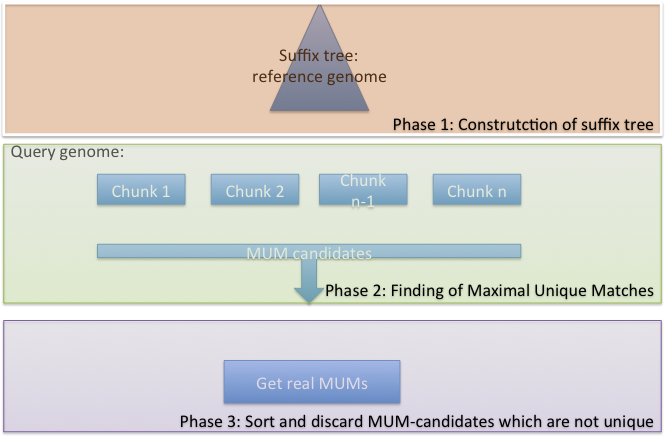
\includegraphics[width=7.5cm,height=5cm]{Phases.png}
\end{center} 
\caption{Find MUMs in multi-core architectures for whole genome alignment.} 
\label{algorithm} 
\end{figure} 
\subsection{The  MUM: an heuristic approach}
Although a pair of conserved genes rarely contain the same entire sequence, they share a lot of short common substrings and some of them are indeed unique to this pair of genes. For example the following two sequences, R and Q:\\
\begin{center}
    R=\underline{ac} ga \underline{ctc} a \underline{gctac} t \underline{ggtcagctatt} \underline{acttaccgc}\$\\
    Q=\underline{ac} tt \underline{ctc} t \underline{gctac} \underline{ggtcagctatt} c \underline{acttaccgc}\$\\
\end{center}
    It is clear that sequences R and Q have many common substrings, they are: ac, ctc, gctac, ggtcagctatt, acttaccgc.\\
Among those five common substrings, ac is the only substring that is not unique. It occurs more than once in both sequences. You can also observe that actually a, c, t, and g are common substrings of R and Q. However, they are not maximal, i.e. they are contained in at least one longer common substrings. We are only interested in those that are of maximal length.\\
Our aim is to search for all these short common substrings. Given genomes R and Q, we need to find all common substrings which are unique and of maximal length. Each of such common substrings is known as Maximum Unique Match (MUM). For almost every conserved gene pairs, there exist at least one MUM which is unique to them.\\
For example, assuming d = 3, sequences R and Q in the previous example has four MUMs: ctc, gctac, ggtcagctatt, acttaccgc. Substring ac is not an MUM because its length is smaller than the value of d and it is not unique to both sequences.
\begin{center}
    R=\xout{ac} ga \sout{ctc} a \uwave{gctac} t \uuline{ggtcagctatt} \uline{acttaccgc}\$\\
    Q=\xout{ac} tt \sout{ctc} t \uwave{gctac} \uuline{ggtcagctatt} c \uline{acttaccgc}\$\\
\end{center}
The concept of MUM is important in whole genome alignment because a significantly long MUM is very likely to be part of the global alignment.
\subsubsection{Finding MUMs in a suffix tree} 
The key idea in this method is to build a suffix tree for genome R, a data structure which allows finding, all distinct subsequences in a given genome.\\
A suffix tree is a data structure which indexes a whole string in every suffix. It allows finding all matches between a reference genome (suffix tree) and a query genome. It can also check for unique matches in the reference very easily just to check if the match ends in a leaf node and by checking the character immediately preceding the start of this match it is possible to determine whether it is a maximal match. To understand the efficient search of matches in a suffix tree, time complexity is $O(m)$ where $m$ is the length of query genome, it is used a suffix link. A link points from a source node $s$ in suffix tree to another destination node $d$ in suffix tree if the string label from the root node to node $d$ is equal to the label from root node to $s$ with the first character removed. In Figure \ref{fig:st} is shown the suffix tree, green lines are suffix links and boxes are start position of every suffix. For instance, the string label of node $i$ in Figure \ref{fig:st} is tgt and next suffix $i+1$ is gt. So that is exactly the tree position corresponding to the next position in the query genome.\\
\begin{figure}
  \centering
  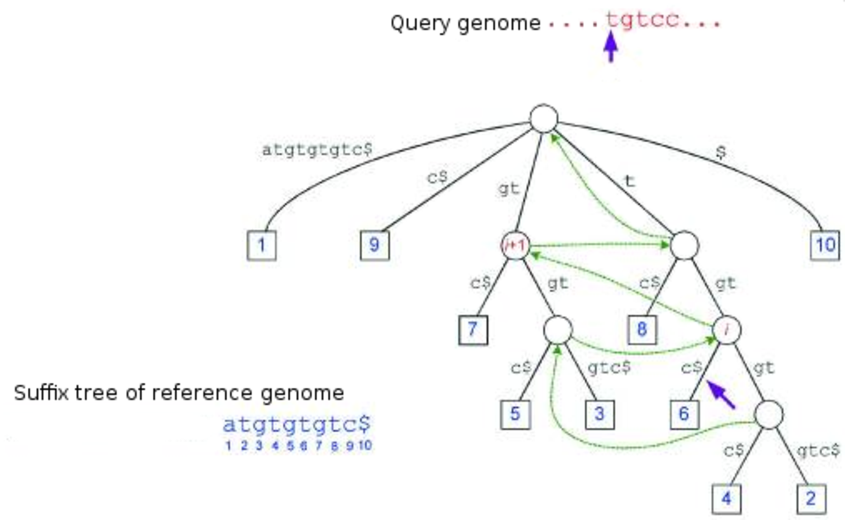
\includegraphics[width=8.5cm,height=5cm]{st-mum.pdf}
  \caption{Suffix tree and its use to find matches between a reference and query genome \cite{Delcher2002}.}
\label{fig:st}
\end{figure}
In Figure \ref{fig:st} the match gtc which starts at $i+1$ in the query genome and node 7 in the suffix tree is not maximal on the left because the preceeding character in both strings is a t.\\
  By construction, the location of a match in the suffix tree represents a substring of the subject sequence which maximaly matches a prefix of
  \texttt{query suffix}. Thus it is only necessary to verify that, the match is long enough, that it is unique in the subject sequence and that 
  the match is also left maximal. This is done as follows:
    \begin{enumerate}
  \item
  Does \texttt{match} represent a substring of lengt h at least \texttt{minimum match length}?
   \item 
  Does \texttt{match} correspond to a leaf edge? Then  then the string represented by the match is unique in the subject sequence.
  \item   
  Is the match left maximal? This is true if one of the following conditions hold:
  \begin{itemize}
  \item   
  The suffix of the query currently considered is the first suffix, or 
  \item 
  The string represented by \texttt{match} is a prefix of the subject string,  or
  \item  
  The characters immediately to the left of the matching strings in the subject sequence and the query sequence are different
  \end{itemize}
  \end{enumerate}
  If all conditions 1-3 are true, then this MUM is stored in a list of MUM-candidates as it is shown in Figure \ref{candidates}. If a match is found but it doesn't reach a leaf node then this match is dropped as it is shown in Figure \ref{candidates}. A MUM-candidate is saved in an array of type MUM-candidate which has the following information:
  \begin{itemize}
    \item Position in reference sequence.
    \item Position in query genome.
    \item Length of match.
  \end{itemize}
 \begin{figure}[htb]  
 \begin{center} 
  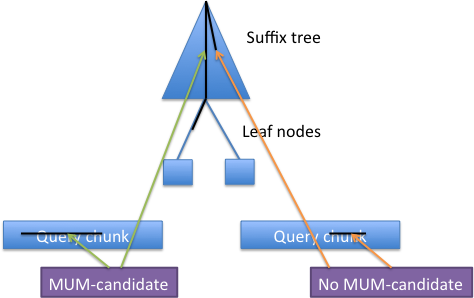
\includegraphics[width=6.5cm,height=4cm]{MUM-candidates.png}
 \end{center} 
 \caption{Finding MUMs in a suffix tree. Blue box represents a leaf node and it saves the start position of its suffix.} 
 \label{candidates} 
 \end{figure}  
 The current serial search method is summarized in Algorithm \ref{alg:find}, the first suffix is \textbf{always} searched from the root node in Suffix Tree and rest of suffixes are searched with suffix links from the node in Suffix Tree from previous search.\\
 \begin{algorithm}
   \caption{MUM search of a query and reference genome.} \label{alg:find}
 \begin{algorithmic}[1]
   \ForAll{Suffix in query genome}
   \State Traversal of suffix tree with current suffix until a mismatch occurs.
   \If{Current match $>$ minimum match length AND Current match is in leaf edge AND Current match is left maximal}
   \State Save Current match as a MUM-candidate. 
   \EndIf
   \If{current node in Suffix Tree is the root node}
   \State Start traversal from root node and from the beginning of current suffix.
   \ElsIf{current node in Suffix Tree is an intermediate node}
   \State Search for suffix link to jump to another node in Suffix Tree.
   \State Continue search of match with rest of suffix from the node which suffix link points out.
   \EndIf
   \EndFor
 \end{algorithmic}
 \end{algorithm}
 MUMs can cover 100\% of the known  conserved gene pairs. Moreover, finding all MUMs  can be done in almost linear time because of the use of suffix links without this artifact we should start every traversal in Suffix Tree from root node adding more execution time because we scan a longer string. Since a Suffix Tree can be queried several times, it is very likely to have more than one query  at the same time. So far, Algorithm \ref{alg:find} is a serial execution because it cannot check for more than one suffix at the same time.
This problem of searching MUM has a time complexity of $O(m+k)$ where $m$ is the length of the query genome and $k$ is the number of maximal unique matches of some minimum length. This problem is a very high intensive computing task, for every substring in the query genome the search for a maximum unique match has to be performed.
\section{Related work}
Search of Maximal Unique Matches to do Whole Genome Alignment was proposed in \cite{Delcher1999}. There have been some previous work in the parallelization of search of matches in genomic data, like \cite{OguzhanKulekci2011,Mongelli,Kouzinopoulos2005}, however these works are focused in fixed patterns and read alignment. On the other hand, there have been achievements in parallelization of Whole genome alignment like \cite{Meng2005}. The parallelization of searching MUMs with a suffix tree is research field not covered very deep, there is only one approach in \cite{Encarnac2011} but without access to source code to check theirs implementation and it is more focused with GPU and CPU hybrid architectures and suffix array.
\section{Parallel algorithm}  
%General-purpose, commodity CPUs currently have SIMD (Single Instruction Multiple Data) functional units and corresponding SIMD instructions. This kind of CPUs allow to be used in several ways of parallel techniques, such as data-level parallelism. \\
%The availability of multi-core architecture makes possible to execute the same task (MUM search) with a different kind of data (chunks of query genome).\\
The sequential version of the MUM search between a reference and query genome trades high computation time when executed in a single machine. \\
Previously the algorithm for sequence alignment was described in detail. Now our own proposal of a parallelization of MUM search within multi-core architecture is explained.\\
There are two resources to improve in this algorithm:
\begin{itemize}
\item Memory usage.
\item CPU.
\end{itemize}
The former was generally improved because it allows being executed in architectures where there is no memory restriction. To improve the performance of the algorithm a data-level parallelism technique is deployed in advance to genome alignment.\\
Our technique is divided in three phases following:
\begin{enumerate}
\item Splitting query genome data (chunks) according to the number of available cores using 1 thread per core.
\item Parallel execution of the task of Algorithm \ref{alg:find} for every chunk then every thread has its own list of MUM-candidates.
\item Get the final list of MUMs from every MUM-candidate list of all threads.
\end{enumerate}
The division of genome data was used using the paradigm of data-level parallelism which consists of a generation of chunks of a query sequence with a fixed size. The chunk size was computed with query genome length divided by number of available threads.\\
The main idea behind using a Maximal Unique Match (MUM): it is possible to cover a huge region of a genome when reference and query genomes are very closely related. However 
to get a MUM, it requires an important feature its uniqueness. 
%We had to face with concept while we evaluated different ways to implement the data-level parallelism. 
Uniqueness can only be found when a whole genome is checked, see Figure \ref{Whole-MUM}. If some part of it is only evaluated we could miss the rest of the genome. In other words, after finding MUMs within a chunk it is not possible to determine if the MUM found is or not a "unique" MUM, globally in the query genome,  because these MUMs are unique only in the chunk that has been read, the rest of the genome it is not known until all query genome has been read. In Figure \ref{Whole-MUM} is shown the consequences of using chunks for query genome. Meanwhile we may speedup the MUM search we need to deal with the discard of MUM-candidates which are not a real MUM. So that, after finding all MUM-candidates for every thread we need to verify which of MUM-candidates are MUM.\\
\begin{figure}[htb]  
\begin{center} 
  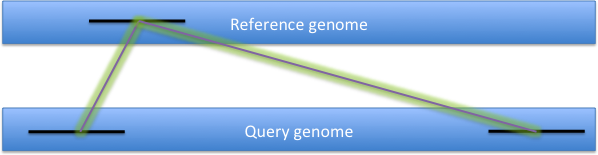
\includegraphics[width=6cm,height=3cm]{Whole-MUM.png}
\end{center} 
\caption{MUM in reference genome but not in query genome.} 
\label{Whole-MUM} 
\end{figure}
In Figure \ref{algorithm} we can see phase 3 which involves to extract the list of MUM from the set of MUM-candidates of every chunk in the query genome. In order to get the real MUMs we filter MUM-candidates that are overlapped by bigger MUM-candidates.\\
\section{Implementation} 
\label{implementation}
\subsection*{Split query genome}  
As it was previously explained, the approach is to use a fixed size division of query genome. To split query genome the algorithm needs to know in advance how many chunks will be used. Then every chunk is computed with two pointers (left and right end) which points out query genome in main memory.
\subsection*{Finding MUMs}
The parallelization is carried out with OpenMP, the Algorithm \ref{alg:find} is applied for every chunk. The algorithm to search MUMs is a process which can be executed without any data dependency. However, when we split a query sequence the following problems arise:
\begin{itemize}
  \item Chunk size is a performance factor.
  \item Different MUM-candidate in query sequence:
    \begin{itemize}
      \item Additional MUMs: this is because we cannot know if the MUM-candidate is unique or not.
      \item Lost MUMs: we may skip MUMs because of the lack of control in pointers to query genome, that is every thread should point to the real value in the query genome.
    \end{itemize}
\end{itemize}
The total number of iterations is the number of chunks created. Every iteration means the whole search of MUMs within a chunk, following the Algorithm \ref{alg:find}, if the right end of chunk is not the end of the query sequence and there are still nucleotides to match then traversal of suffix tree until it occurs a mismatch or a MUM-candidate is found.\\
The key factors in this phase are:
\begin{itemize}
  \item Number of chunks: every chunk is private for each thread.
  \item Size of chunks: delimiters for chunks are private for each thread.
  \item Number of threads.
\end{itemize}
\subsection*{Get real MUMs}
This phase is applied with Algorithm \ref{alg:real} for the set of MUM-candidates. These are ordered with quicksort according to position in query sequence. Every thread has found a set of MUM-candidates from previous phase but all threads don't produce the MUM-candidates in order. That's why a quicksort is required.\\
After quicksort we need to get the real MUMs. A real MUM is unique in the whole reference and query genome. Those MUM-candidates which are overlapped by bigger MUMs are discarded too, see Figure \ref{real-mums} where MUM-candidate in orange colour is discarded because another MUM-candidate has a larger length and they have same match in the reference genome.
%\begin{figure}[htb]  
%\begin{center} 
%  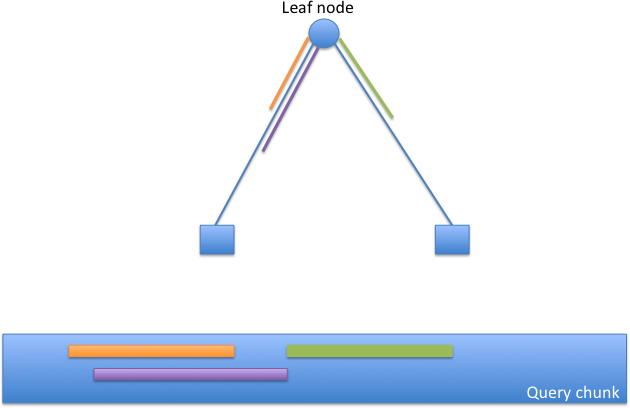
\includegraphics[width=4.5cm,height=4cm]{MUMs.png}
%  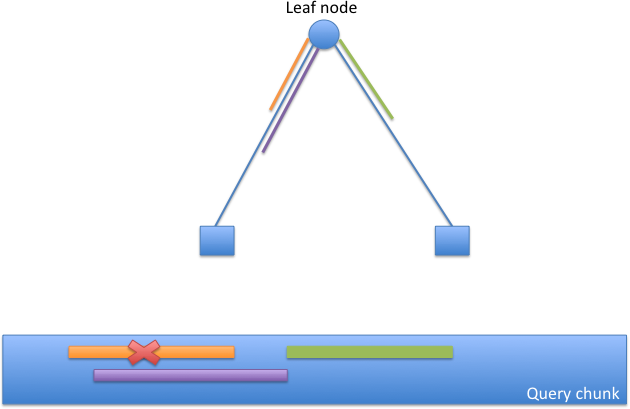
\includegraphics[width=4.5cm,height=4cm]{Remove-MUMs.png}
%\end{center} 
%\caption{Getting Real MUMs.} 
%\label{real-mums} 
%\end{figure}
%The final output has the following format:
%\begin{verbatim} 
%>Information about the query sequence
%Position_in_R Position_in_Q Length_of_MUM
%\end{verbatim}
\section{Experiments and results}
To verify that our approach, can have a better performance to search MUMs of a query and reference genome we check that output of MUMmer and our approach to check that they produce the same MUMs. This test was carried out in the following node:
\begin{itemize}
\item Hardware:  
\begin{itemize}
\item 2 Processor Intel(R) Xeon(R) E5645 @ 2.4GHz of 6 cores each one, 32KB L1 cache, 256KB L2 and 12MB L3 shared cache per socket.
\item RAM: 96 GB
\end{itemize} 
\item  Software: 
\begin{itemize}
\item Linux Kernel 2.6.32-220.el6.x86\_64 \#1 SMP
\item gcc 4.7.0 with OpenMP support
\item PAPI 5.0.1
\end{itemize}  
\item Genomes:
  \begin{itemize}
    \item Reference: Human chromosome 21 single fasta file
    \item Query: Mouse chromosome 16 single fasta file
  \end{itemize}
\end{itemize}
The main objective of the test was to check the performance to search MUMs in multi-core architectures by using OpenMP (threads). The variables to control were:
\begin{enumerate}
  \item Number of chunks for query genome.
  \item Number of threads: from 1 to 24 threads with affinity.
  \item OpenMP scheduling: static with chunk size of 1.
\end{enumerate}
Moreover, the use of Memory Bandwidth was measured with the tool likwid\footnote{Measure hardware performance counters on Intel and AMD processors.}, the use of Memory Bandwidth was checked only in the search of MUMs. The times were collected for the total execution time and the time spent in the parallel region of OpenMP. This parallel region is the algorithm to search MUMs.\\
One key aspect of the several tests deployed was to assure the execution of every thread in a single core, that is no other thread is competing for the same cache. Affinity is a requirement because we need to ensure the scalability of our proposal, without affinity even a number of threads below the number of cores might be in the same core. Affinity ensures us a proper use of performance in a multi-core architecture.\\
The construction of the suffix tree for the reference genome of length 35.45[Mbp] takes 20.66[s] to construct and it uses 608[MB] of memory. The minimum length for a MUM was:20 , 50 and 100 [bp]. The query sequence of length 95.28[Mbp] was divided in chunks equal to the available threads, the total number of MUMs found were 102844 MUMs of minimum length 20[bp], 1410 MUMs of minimum length 50[bp] and 50 MUMs of minimum length 100[bp].\\
Two times were collected during the execution of the experiments: total execution time and execution time to find mums with the function omp\_get\_wtime of OpenMP.\\
Figure \ref{fig:speedup} shows the speedup for the parallelization of searching of MUMs for several minimum lengths of MUM. Moreover from this Figure \ref{fig:speedup} we can conclude that we got a near linear speedup with 12 threads, which is the maximum number of cores. Then there is a reduction in the linear speedup because we start using more than 1 thread per core and this causes a degradation in the phase of searching MUMs. As we can see in Figure \ref{fig:speedup} the better speedup is with a shorter minimum length of MUM and it is a consequence of similarity between our reference and query genome.\\
\begin{figure}[htb]
  \centering
  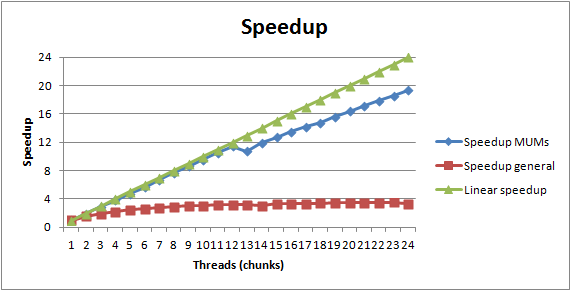
\includegraphics[width=8.5cm,height=5cm]{speedup.png}
  \caption{Speedup of our approach to search MUMs in multi-core architectures with OpenMP.}
  \label{fig:speedup}
 \end{figure}  
 Now we focus in the first experiment to search MUMs of minimum length 20[bp] because it gives more information about the process of searching MUMs. Our goal is to get the best performance of a multicore architecture while searching MUMs and from the Figure \ref{fig:speedup} we can watch a poor performance with more than one thread per core. The reason of this behavior is because the traversal of suffix tree makes the search of MUMs a high intensive memory bound problem. So that the processor is waiting for the next portion of data to traverse the suffix tree. To confirm this idea we measured with PAPI the following counters:
 \begin{itemize}
   \item Total cycles.
   \item Resources stalls.
 \end{itemize}
 From these hardware counters we get the index of stalls for resources in the multi-core architecture with the Formula \ref{eq:stalls}.
 \begin{equation}
   Stalls=\frac{Resources stalls}{Total cycles}
   \label{eq:stalls}
 \end{equation}
 In Figure \ref{fig:stalls} we can confirm that even though the index of stalls is almost the same for different set of threads the index of stalls with 24 threads is almost the same as with only one thread. As a consequence we get a multi-core architecture with a poor performance with more than one thread per core.
 \begin{figure}[htb]
  \centering
  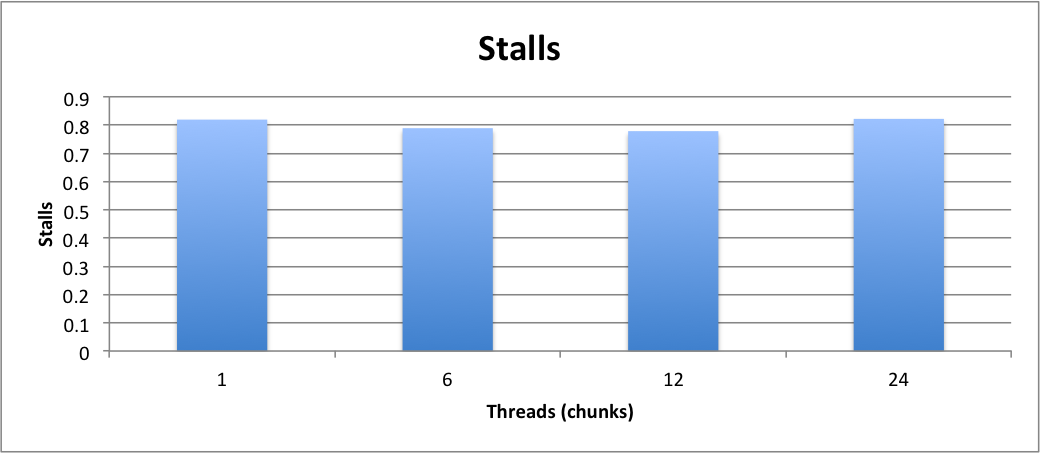
\includegraphics[width=8.5cm,height=5cm]{stalls.png}
  \caption{Resources stalls for search of MUMs of minimum length 20[bp] in multi-core architectures with OpenMP.}
  \label{fig:speedup}
 \end{figure}  
 To improve the performance of our approach the following proposals may be used:
\begin{itemize}
  \item Prefetching: this may work because we know in advance what information from suffix tree and query sequence we need in every traversal of suffix tree. If we can allow the use of some part of suffix tree be stored and read in cache by several threads which request that substree. However, because we use suffix links to jump to another part of suffix tree so that a new part of suffix tree would have to be read.
  \item Explicit cache management: this is a obvious consequence of previous bullet because we may need to store part of the suffix tree in some cache-level of processor.
  \item An improved traversal of suffix tree would improve the overall performance of search of MUMs. So far, one thread traverses the suffix tree if we add multithread traversal of suffix tree to find next edge in the match path we would reduce the execution time.
\end{itemize}
%% \appendix

\section{Conclusions}
This paper presents an evaluation of performance to search MUMs of a query and reference genome in multi-core architectures with OpenMP. The search of MUMs is performed in a suffix tree and the list of MUMs can help in the process of whole genome alignment. The results shows that the heaviest section of searching MUMs in a suffix tree is improved with the use of a multi-core architecture. Although we got a near linear speedup with only one thread per core, there is more improvements to do. These improvements involve a better use of resources (memory and CPU) when we have more than thread per core. In spite of suffix tree is a good data structure to string matching, when is used in multi-core architectures it shows a slow performance (high CPI) to search MUMs.\\
From the results obtained we conclude that bottleneck is in our data structure: suffix tree. We require to handle a strategy to traverse a suffix tree in multi-core architectures, this approach only queries the suffix tree for one string at a time. However, the traversal of suffix tree is still done in a serial way.
%% \label{}

\section*{Acknowledgements}
This work was supported by grant from Ejecuci\'on eficiente de aplicaciones multidisciplinares: nuevos desaf\'ios en la era multi/many core, with reference TIN2011-28689-C02-01.
%% References
%%
%% Following citation commands can be used in the body text:
%% Usage of \cite is as follows:
%%   \cite{key}         ==>>  [#]
%%   \cite[chap. 2]{key} ==>> [#, chap. 2]
%%

%% References with BibTeX database:
\section*{References}
\bibliographystyle{elsarticle-num}
\bibliography{mum-multithread}

\end{document}

%%
%% End of file `procs-template.tex'. 
